$$
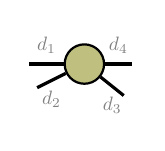
\begin{tikzpicture}[baseline=-0.5ex]
    \tikzset{tensor/.style = {minimum size = 0.5cm,shape = circle,thick,draw=black,inner sep = 0pt}, edge/.style = {thick,line width=.4mm},every loop/.style={}}
    \def\x{6}
    \def\y{0}
     \node[tensor,fill=green!50!red!50!white] (B) at (\x+1,\y) {$\St$};
    \draw[edge] (B) -- (\x+0.3,0) node [midway,above] {\scalebox{0.7}{\textcolor{gray}{$d_1$}}};
    \draw[edge] (B) -- (\x+1.6,0) node [midway,above] {\scalebox{0.7}{\textcolor{gray}{$d_4$}}};;
    \draw[edge] (B) -- (\x+0.4,-0.3) node [midway, below] {\scalebox{0.7}{\textcolor{gray}{$d_2$}}};;
    \draw[edge] (B) -- (\x+1.5,-0.4)node [midway, below] {\scalebox{0.7}{\textcolor{gray}{$d_3$}}};;
\end{tikzpicture}=
\begin{tikzpicture}[baseline=\baseline]
    \tikzset{tensor/.style = {minimum size = 0.5cm,shape = circle,thick,draw=black,inner sep = 0pt}, edge/.style   = {thick,line width=.4mm},every loop/.style={}}
    \def\y{0}
    \def\x{0}
  \node[tensor,fill=red!30!white] (D) at (\x-1,\y){$\Gt_1$};
  \node[tensor,fill=red!50!white] (A) at (\x,\y){\scalebox{0.85}{$\Gt_2$}};
  \node[tensor,fill=blue!50!white] (B) at (\x+1,\y){$\Gt_3$};
   \node[tensor,fill=blue!20!white] (C) at (\x+2,\y){$\Gt_4$};
    \draw[edge](A) -- (\x,\y-0.7)node [midway,left] {\edgelabel{$d_2$}};
    \draw[edge](B) -- (\x+1,\y-0.7)node [midway,left] {\edgelabel{$d_3$}};
    \draw[edge](C) -- (\x+2,\y-0.7)node [midway,left] {\edgelabel{$d_4$}};
     \draw[edge](D) -- (\x-1,\y-0.7)node [midway,left] {\edgelabel{$d_1$}};
    \draw[edge](D) -- (A) node [midway,above] {\edgelabel{$R_1$}};
    \draw[edge](A) -- (B) node [midway,above] {\edgelabel{$R_2$}};
    \draw[edge](B) -- (C) node [midway,above] {\edgelabel{$R_3$}};
\end{tikzpicture}.
$$
The TT decomposition was initially introduced in the quantum physics and condensed matter community as \emph{Matrix Product States~(MPS)}. In this context, the dimensions of the internal edges are referred to as \textit{bond dimensions}, and the free legs are called \textit{physical dimensions}.
Next, we show how an exact TT decomposition of a tensor $\St\in\RR^{d_1\times\dots\times d_N}$ can be computed in polynomial time using successive singular value decomposition (SVD). This algorithm is known as the TT-SVD algorithm~\citep{oseledets2010approximation}, but was introduced earlier in the quantum physics community and referred to as \textit{successive Schmidt decompositions}~\citep{vidal2004efficient,mcculloch2007density}. 
Before presenting the TT-SVD algorithm, we introduce the notions of left and right orthogonality for third-order tensors.
\begin{definition}\label{def:left-right-ortho}A core tensor $\At_n\in\RR^{R_{n-1}\times d_n\times R_n}$ for $n\in[N]$ is left-orthogonal if $(\At_n)_{(3)}^\ts(\At_n)_{(3)}=\Ib_{R_n}$ and right-orthogonal if $(\At_n)_{(1)}(\At_n)_{(1)}^\ts=\Ib_{R_{n-1}}$. This can be illustrated using tensor networks 
as follows:
\begin{align*}
\begin{tikzpicture}[baseline=\baseline]
    \tikzset{tensor/.style = {minimum size = 0.5cm,shape = circle,thick,draw=black,inner sep = 0pt}, edge/.style = {thick,line width=.4mm},every loop/.style={}}
    \def\y{0}
    \def\x{0}
    \node[tensor, path picture={
    \fill[fill=red!30!white](path picture bounding box.south east)
        -- 
    (path picture bounding box.north west) --
    (path picture bounding box.north east) -- cycle;
    }, shift={(\x,\y)}] (A) {\scalebox{0.85}{$\At_n$}};
    \draw[edge](A) -- (\x,\y-0.7)node [midway,left] {\scalebox{0.7}{\dimcolor{$d_n$}}};
    \draw[edge](A) -- (\x-0.85,\y)node [midway,above] {\scalebox{0.7}{\dimcolor{$R_{n-1}$}}};
    \draw[edge](A) -- (\x+0.85,\y)node [midway,above] {\scalebox{0.7}{\dimcolor{$R_n$}}};
\end{tikzpicture}\ \  \text{is left-orthogonal}
\iff
\begin{tikzpicture}[baseline=\baseline]
    \tikzset{tensor/.style = {minimum size = 0.5cm,shape = circle,thick,draw=black,inner sep = 0pt}, edge/.style = {thick,line width=.4mm},every loop/.style={}}
    \def\y{0}
    \def\x{0}
    \node[tensor, path picture={
    \fill[fill=red!30!white](path picture bounding box.south west)
        -- 
    (path picture bounding box.north east) --
    (path picture bounding box.north west) -- cycle;
    }, shift={(\x,\y)}] (A1) {\scalebox{0.85}{$\At_n$}};
    \node[tensor, path picture={
    \fill[fill=red!30!white](path picture bounding box.south east)
        -- 
    (path picture bounding box.north west) --
    (path picture bounding box.north east) -- cycle;
    }, shift={(\x+1,\y)}] (A2) {\scalebox{0.85}{$\At_n$}};
    \draw[edge](A1)--(A2)node [midway,above] {\scalebox{0.7}{\dimcolor{$R_{n-1}$}}};
    \draw[edge](\x+0.23,\y-0.1) -- (\x+0.77,\y-0.1) node [midway,below] {\scalebox{0.7}{\dimcolor{$d_n$}}};
    \draw[edge](A1) -- (\x-0.85,\y)node [midway,above] {\scalebox{0.7}{\dimcolor{$R_{n}$}}};
    \draw[edge](A2) -- (\x+1.85,\y)node [midway,above] {\scalebox{0.7}{\dimcolor{$R_{n}$}}};
\end{tikzpicture}
=
\begin{tikzpicture}[baseline=\baseline]
    \tikzset{tensor/.style = {minimum size = 0.5cm,shape = circle,thick,draw=black,inner sep = 0pt}, edge/.style = {thick,line width=.4mm},every loop/.style={}}
    \def\y{0}
    \def\x{0}
    \draw[edge](\x,\y) -- (\x+1.5,\y)node [midway,above] {\scalebox{0.7}{\dimcolor{$R_n$}}};
\end{tikzpicture}=\Ib_{R_n},
\end{align*}
similarly,
\begin{align*}
\begin{tikzpicture}[baseline=\baseline]
    \tikzset{tensor/.style = {minimum size = 0.5cm,shape = circle,thick,draw=black,inner sep = 0pt}, edge/.style = {thick,line width=.4mm},every loop/.style={}}
    \def\y{0}
    \def\x{0}
    \node[tensor, path picture={
    \fill[fill=blue!30!white](path picture bounding box.south west)
        -- 
    (path picture bounding box.north east) --
    (path picture bounding box.north west) -- cycle;
    }, shift={(\x,\y)}] (A) {\scalebox{0.85}{$\At_n$}};
    \draw[edge](A) -- (\x,\y-0.7)node [midway,left] {\scalebox{0.7}{\dimcolor{$d_n$}}};
    \draw[edge](A) -- (\x-0.85,\y)node [midway,above] {\scalebox{0.7}{\dimcolor{$R_{n-1}$}}};
    \draw[edge](A) -- (\x+0.85,\y)node [midway,above] {\scalebox{0.7}{\dimcolor{$R_n$}}};
\end{tikzpicture}\ \  \text{is right-orthogonal}
\iff
\begin{tikzpicture}[baseline=\baseline]
    \tikzset{tensor/.style = {minimum size = 0.5cm,shape = circle,thick,draw=black,inner sep = 0pt}, edge/.style = {thick,line width=.4mm},every loop/.style={}}
    \def\y{0}
    \def\x{0}
    \node[tensor, path picture={
    \fill[fill=blue!30!white](path picture bounding box.south west)
        -- 
    (path picture bounding box.north east) --
    (path picture bounding box.north west) -- cycle;
    }, shift={(\x,\y)}] (A1) {\scalebox{0.85}{$\At_n$}};
    \node[tensor, path picture={
    \fill[fill=blue!30!white](path picture bounding box.south east)
        -- 
    (path picture bounding box.north west) --
    (path picture bounding box.north east) -- cycle;
    }, shift={(\x+1,\y)}] (A2) {\scalebox{0.85}{$\At_n$}};
    \draw[edge](A1)--(A2)node [midway,above] {\scalebox{0.7}{\dimcolor{$R_{n}$}}};
    \draw[edge](A1) -- (\x-0.85,\y)node [midway,above] {\scalebox{0.7}{\dimcolor{$R_{n-1}$}}};
    \draw[edge](A2) -- (\x+1.85,\y)node [midway,above] {\scalebox{0.7}{\dimcolor{$R_{n-1}$}}};
    \draw[edge](\x+0.23,\y-0.1) -- (\x+0.77,\y-0.1) node [midway,below] {\scalebox{0.7}{\dimcolor{$d_n$}}};
\end{tikzpicture}
=
\begin{tikzpicture}[baseline=\baseline]
    \tikzset{tensor/.style = {minimum size = 0.5cm,shape = circle,thick,draw=black,inner sep = 0pt}, edge/.style = {thick,line width=.4mm},every loop/.style={}}
    \def\y{0}
    \def\x{0}
    \draw[edge](\x,\y) -- (\x+1.5,\y)node [midway,above] {\scalebox{0.7}{\dimcolor{$R_{n-1}$}}};
\end{tikzpicture}=\Ib_{R_{n-1}}.
\end{align*}
\end{definition}
The following theorem establishes the existence of a minimal tensor train decomposition for any tensor, and its proof is constructive, outlining the TT-SVD algorithm.
\begin{theorem}(\textbf{Computing (Orthogonal) Tensor Train Decomposition.})\label{thm:tt-decomposition}
For any $\St\in\RR^{d_1\times\dots\times d_N}$, let $\St_{([n])}\in\RR^{d_1\dots d_n\times d_{n+1}\dots d_N}$ be the matricization obtained by mapping the first $n$  modes of $\St$ to the rows of $\St_{[n]}$. Then the TT rank $(R_1,\cdots,R_{N-1})$ of $\St$  is given
by
    $R_n = \rank~(\St_{([n])})$ for all $n\in[N-1]$.
\end{theorem}
\begin{proof}
    Let $R_n = \rank~(\St_{([n])})$. We first show that we can construct a TT decomposition of $\St\in\RR^{d_1\times\cdots\times d_N}$ of rank $(R_1,R_2,\cdots,R_{N-1})$ by successive QR decomposition. For simplicity, we consider the case $N=4$, but the argument can easily be generalized.

